\problemname{G: Cordon Bleu}
\balloon{231f20}

\begin{center}
% Mix of two public domain cliparts
 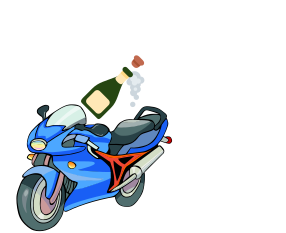
\includegraphics[width=4cm]{cordon_bleu.pdf}
 \end{center}

\noindent
A Parisian entrepreneur has just opened a new restaurant
``Au~bon~cordon~bleu'',
named after a famous French recipe.  However, no one has any
idea of which wine would be appropriate with such a dish. The entrepreneur
plans to sample many different wines in order to build the wine menu.

The various bottles of wine he plans to taste can be obtained from
different wine merchants located in or around Paris. Being a very
sensitive product, high-quality wine can only be transported by highly
trained couriers on motorbikes. Therefore, those couriers are very expensive.

A courier can be used for the transportation of several wine bottles,
but can transport only one bottle at a time. All couriers get paid
at the same fixed rate: one euro per kilometer. The distance function
used is the Manhattan distance (also known as taxicab metric)
of every individual segment of the trip:
the distance from a point $(x_1, y_1)$ to a point $(x_2, y_2)$ is
$|x_1-x_2|+|y_1-y_2|$.

A courier in charge of transporting a single wine bottle will
get paid as many euros as the sum of the following two (Manhattan) distances:
from her base to the wine merchant place, and from the wine merchant
place to the restaurant.

Consider a more complex example: a courier in charge of transporting two wine
bottles, one after the other. The amount paid will be the sum of the
following distances: from his base to the location of the first bottle,
then to the restaurant, then to the location of the second bottle, then to
the restaurant.

Help the entrepreneur
minimize the costs of hiring the couriers. Given a set of Cartesian
coordinates corresponding to available couriers, a set of Cartesian
coordinates corresponding to the locations of the precious wine bottles
they need to collect, and the location of the restaurant,
compute the smallest number of kilometers that the couriers will be
paid for.  There is no obligation to use all available
couriers, and bottles can be collected in an arbitrary order.

\subsection*{Input}

The input comprises several lines, each consisting of integers
separated with single spaces:
\begin{itemize}
\item The first line consists of the number $N$ of
wine bottles to collect and the number  $M$
of available couriers.

\item The $N$ following lines consist of the coordinates of each bottle as
two integers $x$ and $y$.

\item The $M$ following lines consist of the coordinates of each
  courier's base
as two integers $x$ and $y$.

\item The last line contains the coordinates of the restaurant as two
  integers $x$ and $y$.
\end{itemize}

\subsection*{Limits}
\begin{itemize}
  \item $1 \leq N \leq 1\,000$;
  \item $1 \leq M \leq 1\,000$;
  \item all coordinates $(x,y)$ verify $-1\,000 \leq x \leq 1\,000$ and
$-1\,000 \leq y \leq 1\,000$.
\end{itemize}

\subsection*{Output}

A single integer: the smallest number of euros that needs to be
paid to collect all bottles.


\subsection*{Notes}

There might be more than one item at the same initial location. For
example, it would be possible for two bottles, ten couriers, and the
restaurant to share the same starting position.

\subsection*{Example}

\begin{center}
  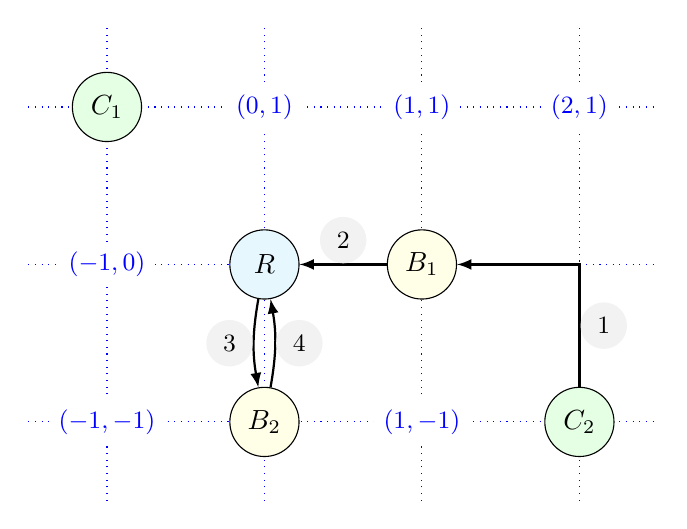
\begin{tikzpicture}[scale=2]
    \tikzset{->,>=latex,circle,
      item/.style={draw,minimum width=2.5em},
      bottle/.style={item,fill=yellow!10},
      courier/.style={item,fill=green!10},
      restaurant/.style={item,fill=cyan!10},
      label/.style={fill=gray!10,minimum width=.2em,midway},
      coord/.style={thin,blue,fill=white,rectangle,-}};
    \draw[coord,dotted] (-1.5, -1.5) grid (2.5, 1.5);
    \node[coord] at (-1,-1) { \small $(-1,-1)$ };
    \node[coord] at (1,-1) { \small $(1,-1)$ };
    \node[coord] at (-1,0) { \small $(-1,0)$ };
    \node[coord] at (0,1) { \small $(0,1)$ };
    \node[coord] at (1,1) { \small $(1,1)$ };
    \node[coord] at (2,1) { \small $(2,1)$ };
    \node[courier] (C1) at (-1,1) { $C_1$ };
    \node[courier] (C2) at (2,-1) { $C_2$ };
    \node[bottle] (B1) at (1,0) { $B_1$ };
    \node[bottle] (B2) at (0,-1) { $B_2$ };
    \node[restaurant] (R) at (0,0) { $R$ };
    \draw[thick] (C2) |- (B1) node[label,near start,anchor=west]{\small 1};
    \draw[thick] (B1) -- (R) node[label,anchor=south]{\small 2};
    \draw[thick] (R) to[bend right=10] node[label,anchor=east]{\small 3} (B2);
    \draw[thick] (B2) to[bend right=10] node[label,anchor=west]{\small 4} (R);
  \end{tikzpicture}
\end{center}

\noindent 
On this example, only one courier ($C_2$) is used to retrieve the two
bottles $B_1$ and $B_2$, and bring them to the restaurant $R$ by performing
the moves labeled 1 to 4 in succession. The total number of kilometers is 5. This is one of the optimal solutions.
